\usetheme{metropolis}

\usepackage{appendixnumberbeamer}

\usepackage{booktabs}
\usepackage[scale=2]{ccicons}

\usepackage{pgfplots}
\usepgfplotslibrary{dateplot}

\usepackage{xspace}
\newcommand{\themename}{\textbf{\textsc{metropolis}}\xspace}

\metroset{titleformat frame=smallcaps}

% Add section numbers in TOC
% https://tex.stackexchange.com/a/44998/173708
\setbeamertemplate{section in toc}[sections numbered]

%%% Local Variables:
%%% mode: latex
%%% TeX-master: t
%%% End:


% make background color for title of the slides green
\definecolor{OilGainsGreen}{RGB}{85, 130, 5}    % Fidelity green normal
\setbeamercolor{frametitle}{bg=OilGainsGreen}   % do not change foreground color

\graphicspath{{figs/}}
% % Figure placement using textpos
% \usepackage{graphicx}
% \usepackage[absolute,overlay]{textpos}
% \setlength{\TPHorizModule}{1cm}
% \setlength{\TPVertModule}{1cm}
% \def\placefig#1#2#3#4{\begin{textblock}{.1}(#1,#2)\rlap{\includegraphics[#3]{#4}}\end{textblock}}
% 
% \def\maxwidth{11.5cm}
% \def\maxheight{8cm}
% % Scale images if necessary, so that they will not overflow the page
% % margins by default, and it is still possible to overwrite the defaults
% % using explicit options in \includegraphics[width, height, ...]{}
% \setkeys{Gin}{width=\maxwidth,height=\maxheight,keepaspectratio}
% 
% \def\fullwidth#1{\vspace*{-0.2cm}\par\centerline{\includegraphics[width=20cm]{#1}}}
% \def\fullheight#1{\vspace*{-0.2cm}\par\centerline{\includegraphics[height=12cm]{#1}}}

% % this works but partially extends
% \titlegraphic{%
%   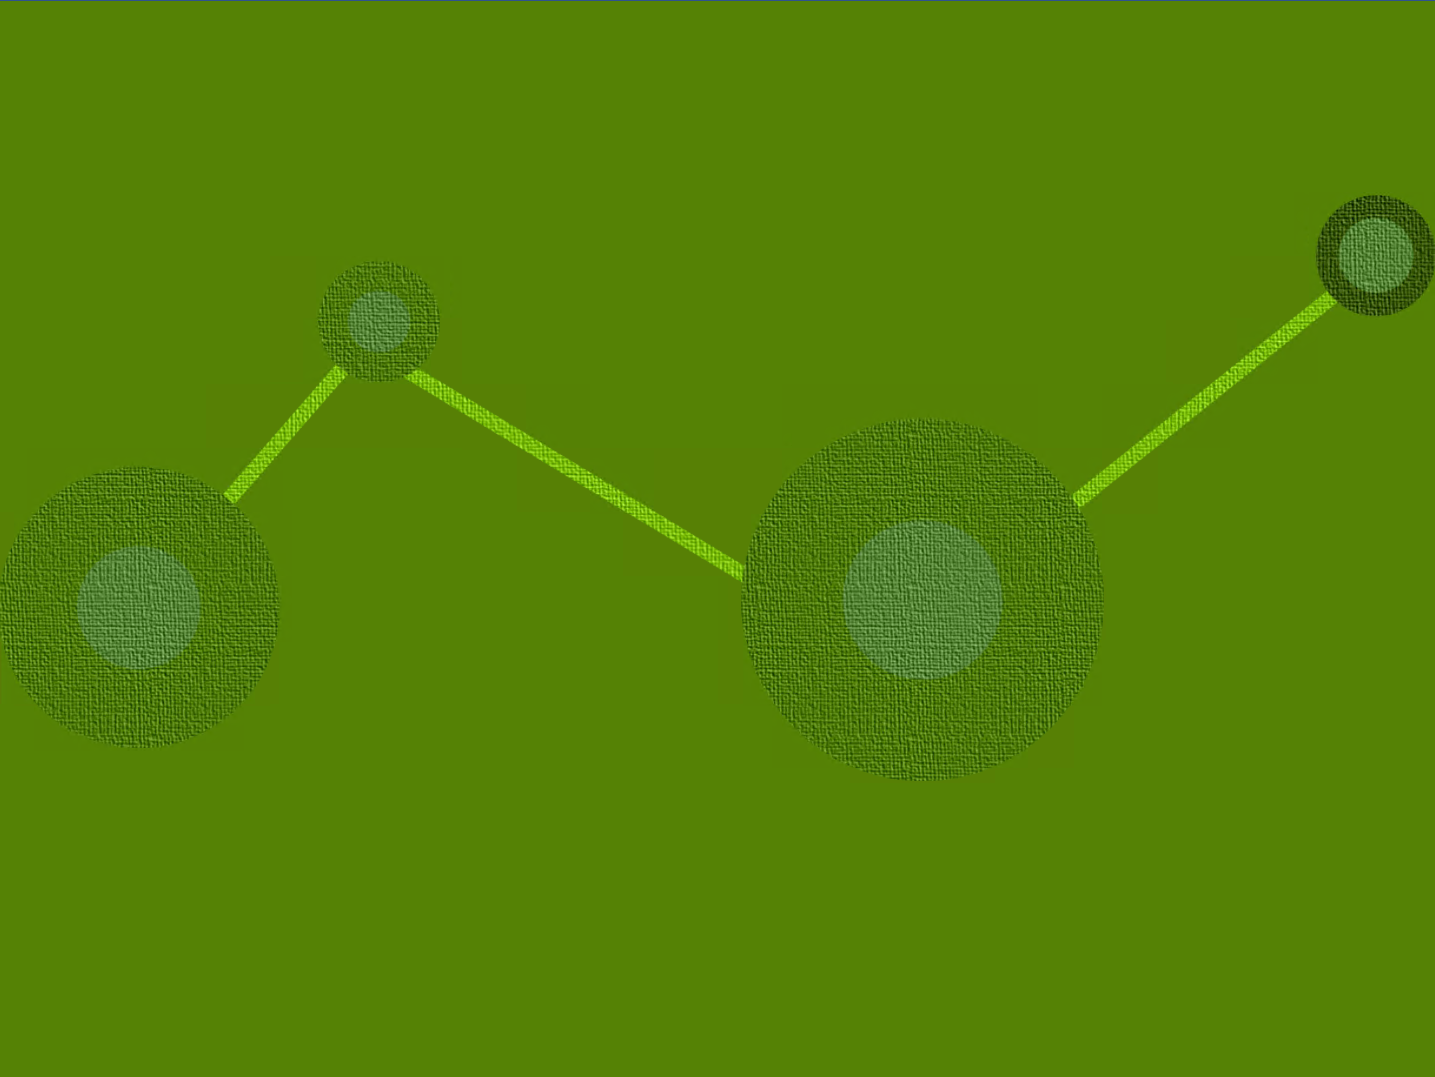
\includegraphics[width=\paperwidth,height=\paperheight]{OilGainsTitleSlide2}
% }

% % https://tex.stackexchange.com/a/412707/173708
% \titlegraphic{%
%   \begin{picture}(0,0)
%     \put(300,10){\makebox(0,0)[rt]{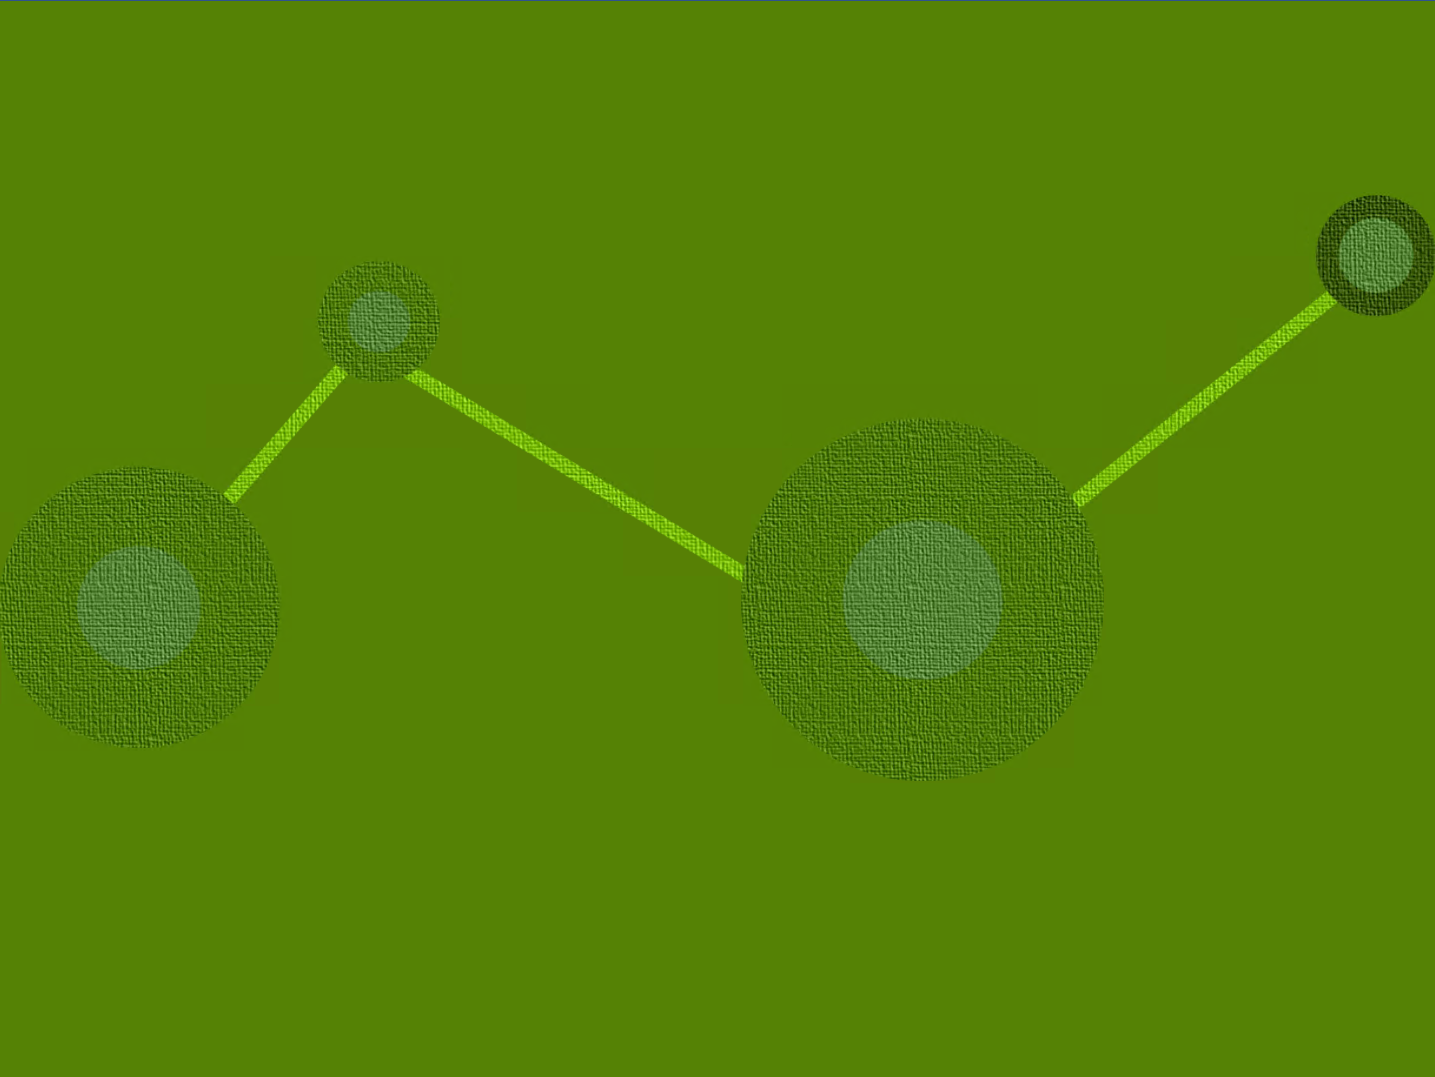
\includegraphics[width=12cm]{OilGainsTitleSlide2}}}
%   \end{picture}}

% remove the [rt] keyword. Offset and increase to maximum size
% https://tex.stackexchange.com/a/412707/173708
\titlegraphic{%
  \begin{picture}(0,0)
    \put(154,-114){\makebox(0,0){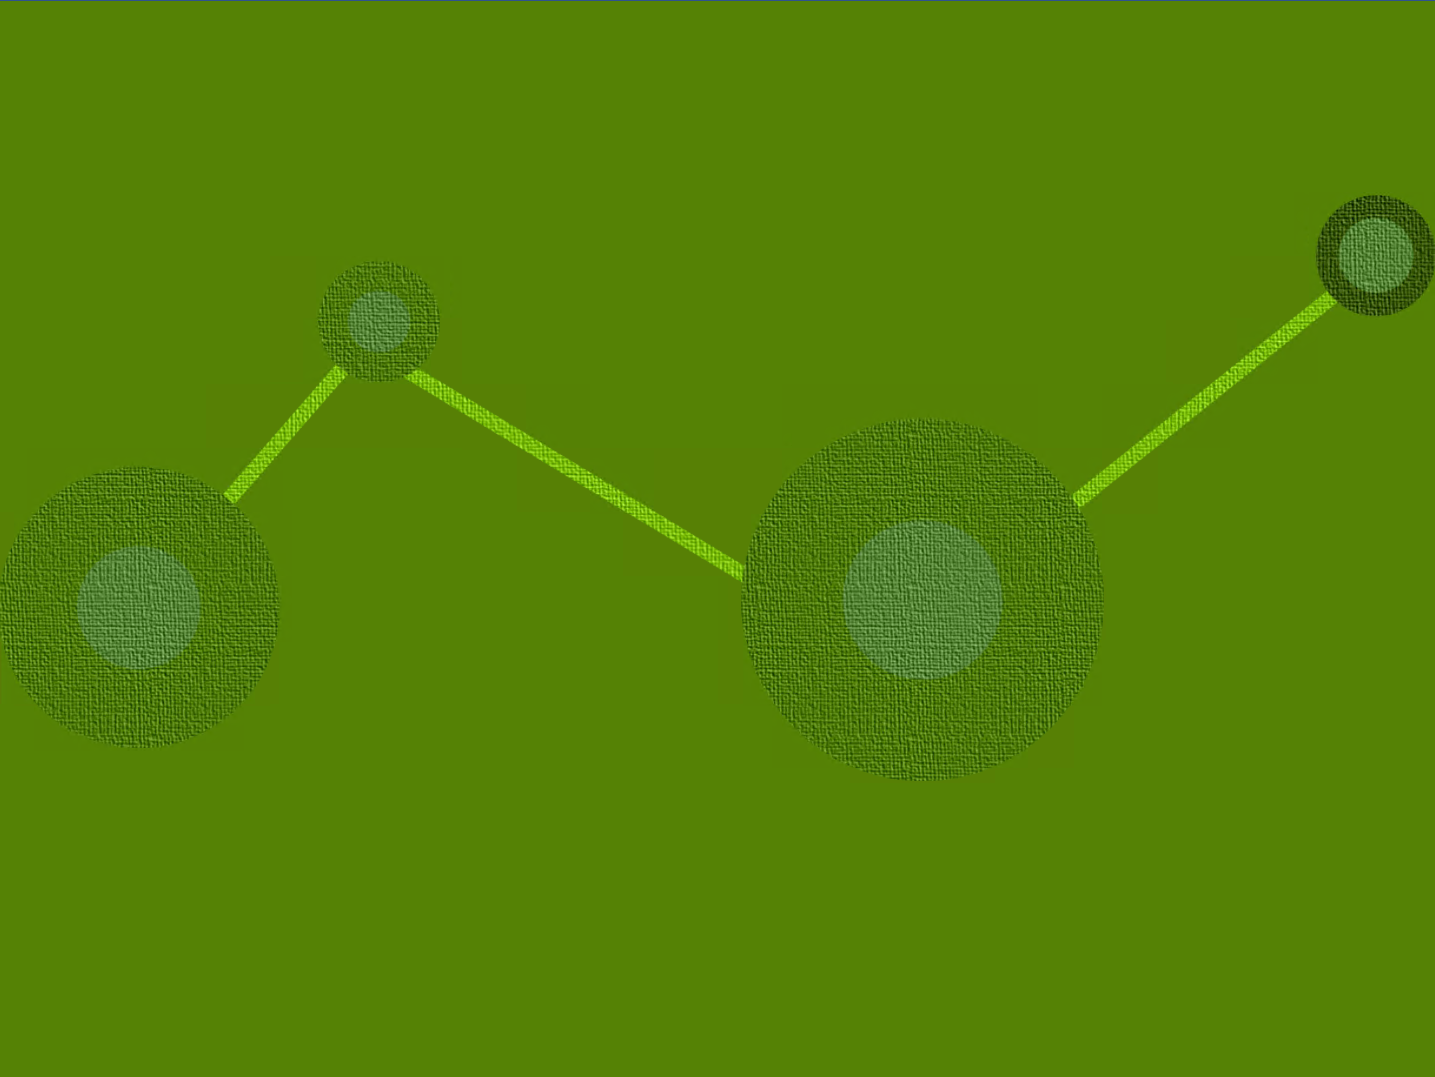
\includegraphics[width=\paperwidth,height=\paperheight]{OilGainsTitleSlide2}}}
  \end{picture}}


% Title Slide here: png file under figs folder
% {\placefig{-0.01}{-0.01}{width=1.01\paperwidth,height=1.01\paperheight}{OilGainsTitleSlide2}


% % this works as a transparent background but overlaps text
% \setbeamertemplate{title page}{\tikz[remember picture,overlay]\node[opacity=0.3] at (current page.center) {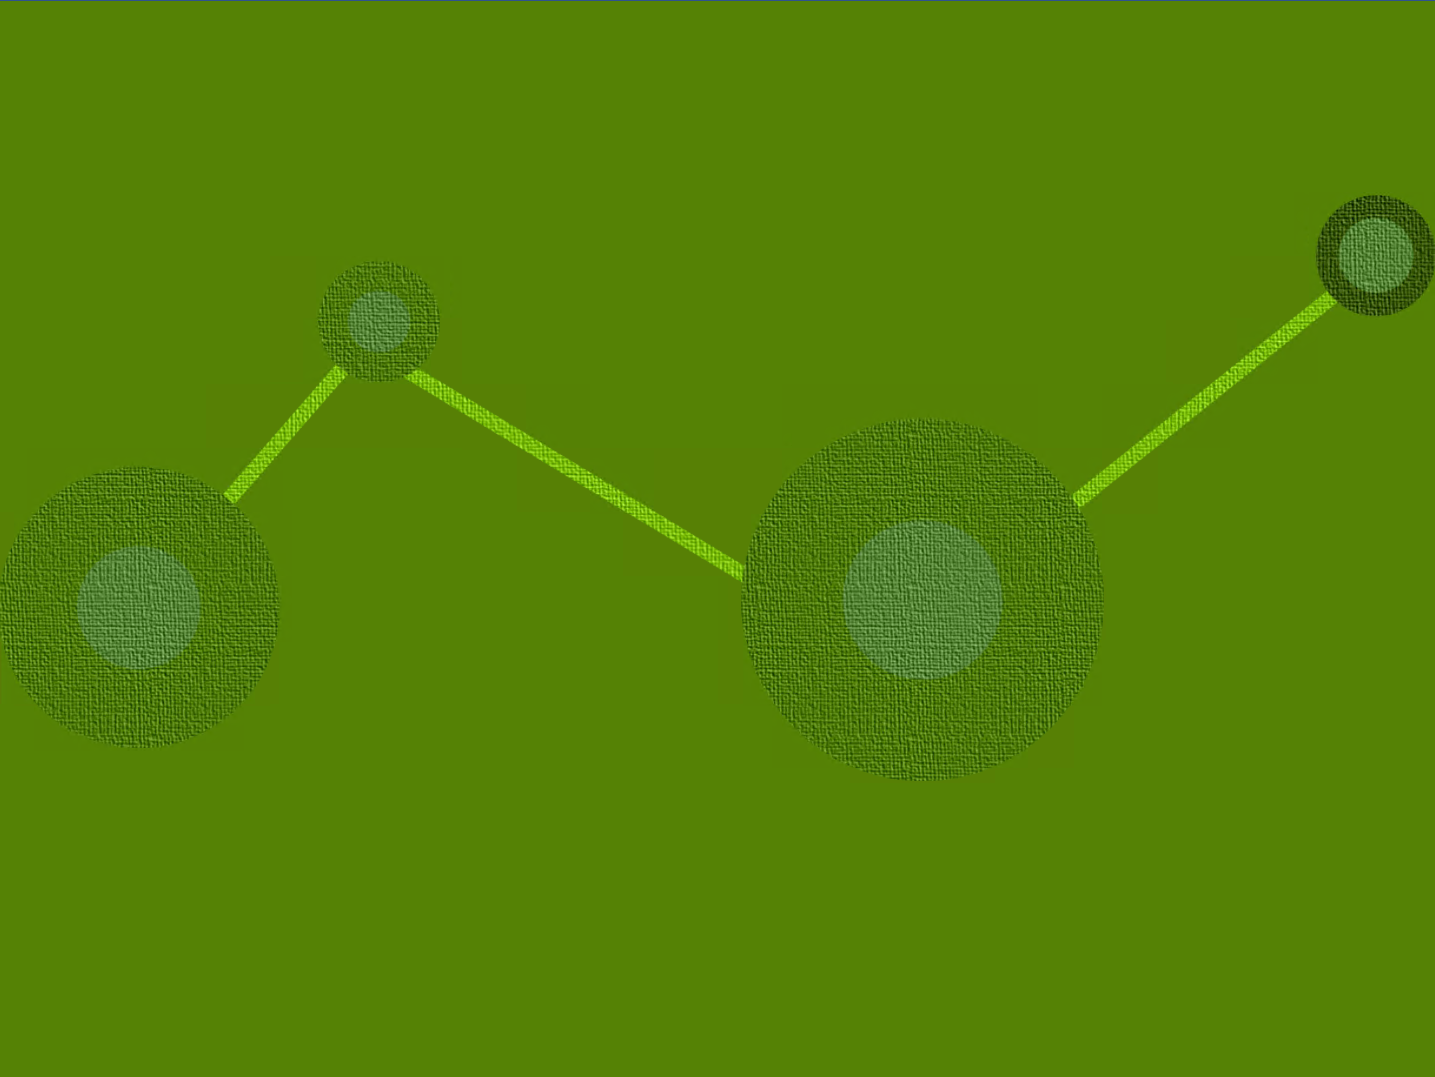
\includegraphics[width=\paperwidth,height=\paperheight,keepaspectratio]{OilGainsTitleSlide2}};}

% change color of title and subtitle
\definecolor{OilGainsGreen}{RGB}{85, 130, 5}  % Fidelity green normal
\setbeamercolor{title}{fg=white,bg=OilGainsGreen}
\setbeamercolor{subtitle}{fg=yellow,bg=OilGainsGreen}
\setbeamercolor{author}{fg=white,bg=OilGainsGreen}
\setbeamercolor{date}{fg=white,bg=OilGainsGreen}
\setbeamercolor{institute}{fg=yellow,bg=OilGainsGreen}
